\documentclass{article}

\usepackage{times}
\usepackage{geometry}
\geometry{a4paper,left=0.6cm,right=0.7cm,top=1.5cm,bottom=1cm,columnsep=0.8cm}

\usepackage{fontawesome}          % icônes de base seulement
\usepackage[hidelinks]{hyperref}
\usepackage{multicol}
\usepackage{tikz}
\usepackage{hyphsubst}
\usepackage{moresize}
\usepackage{hyphenat}
\usepackage{tabularx}
\usepackage{ragged2e}
\usepackage{xcolor}
\usepackage{enumitem}
\usetikzlibrary{calc, positioning}
\newcolumntype{Y}{>{\RaggedRight\arraybackslash}X}

% icônes manquantes -> puce
\makeatletter
\@for\sym:=faBrain,faMicrochip,faHandshakeO,faTools,faNetworkWired,%
             faDatabase,faServer,faGit,faUsers,faComments,faCalendar,faGroup\do{%
  \@ifundefined{\sym}{\expandafter\newcommand\csname\sym\endcsname{\textbullet}}{}}
\makeatother

% couleurs
\definecolor{maincolor}{HTML}{f0fafc}
\definecolor{seccolor}{HTML}{ffffff}
\definecolor{gray}{HTML}{8c94a9}
\definecolor{sidetext}{HTML}{59cee5}

% bande latérale bleue
\usepackage{eso-pic}
\AddToShipoutPictureBG{%
  \begin{tikzpicture}[remember picture,overlay]
    \fill[maincolor] (current page.north west) rectangle
                     ([xshift=0.3\paperwidth] current page.south west);
  \end{tikzpicture}%
}

% listes
\setlist[itemize]{itemsep=-2pt,topsep=0pt,leftmargin=1.08cm}
\renewcommand{\labelitemi}{\textcolor{sidetext}{\footnotesize$\bullet$}}

\setlength{\parindent}{0pt}
\usepackage{paracol}
\columnratio{0.3}

\begin{document}
\pagestyle{empty}

\begin{paracol}{2}
% ────────────────────────────────────────
% Colonne gauche
% ────────────────────────────────────────
\color{sidetext}
\vspace*{-0.5cm}

\noindent
\begin{minipage}{\linewidth}
  \centering
  \begin{tikzpicture}
    \clip (0,0) circle (1.5cm) node[anchor=center]
      {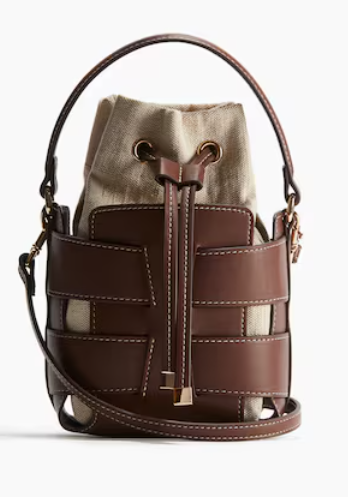
\includegraphics[width=3cm]{0283e106742a4bd8910a7f25041348e9.png}};
  \end{tikzpicture}

  \vspace{3mm}
  {\color{black}\LARGE \textbf{Judikael MOUROUVIN}}

  \vspace{1mm}
  {\large Alternant en marketing digital \& support informatique}

  \vspace{3mm}
  {\color{gray}\rule{\linewidth}{0.4pt}} \\
\end{minipage}

% ── Coordonnées
\begin{tabular}{@{}c l}
  \faPhone &
  \begin{tabular}[t]{@{}l@{}}
    {\color{gray}Téléphone} \\ +590 0690 91 14 48
  \end{tabular} \\
  \\
  \faLinkedin &
  \begin{tabular}[t]{@{}l@{}}
    {\color{gray}LinkedIn} \\
    \href{}{Mon LinkedIn}
  \end{tabular} \\
  \\
  \faMapMarker &
  \begin{tabular}[t]{@{}l@{}}
    {\color{gray}Adresse} \\ Route de Cocoyer \\ 97190 Le Gosier
  \end{tabular} \\
  \\
  \faEnvelope &
  \begin{tabular}[t]{@{}l@{}}
    {\color{gray}Email} \\
    \href{mailto:jkmou971@gmail.com}{jkmou971@gmail.com}
  \end{tabular} \\
\end{tabular}

\vspace{2mm}
{\color{gray}\rule{\linewidth}{0.4pt}} \\

% ── Langues --------------------------------------------------------
{\color{black}{Langues}}

\vspace{2mm}
\begin{itemize}[leftmargin=*]
\item Anglais - \textcolor{gray}{}
\item Espagnol - \textcolor{gray}{}\end{itemize}          % ← le placeholder va contenir \begin{itemize}…\end{itemize}

{\color{gray}\rule{\linewidth}{0.4pt}} \\

% ── Compétences ----------------------------------------------------
\vspace{2mm}
{\color{black}{Compétences Clés}}

\vspace{2mm}
\begin{itemize}[leftmargin=*]
\item Administration
\item Maintenance
\item Réseaux
\item Support
\item Marketing
\item Digital
\item Diagnostic\end{itemize}              % ← idem, une vraie liste
\vspace{2mm}
{\color{gray}\rule{\linewidth}{0.4pt}} \\

% ── Centres d'intérêt
\vspace{2mm}
{\color{black}{Centres d’intérêt}}

\vspace{2mm}
\begin{itemize}[leftmargin=*]
\item Lectur
\item Sports
\item Musique
\item Voyage
\end{itemize}     % ← simple itemize ou tabular

\vfill
~

% ────────────────────────────────────────
\switchcolumn
% Colonne droite
% ────────────────────────────────────────
\color{black}

% ── Profil
\textcolor{black}{\Large \textbf{Profil Professionnel}} \\[2pt]
Passionné d’informatique et de marketing digital, j’ai développé de solides compétences en administration de systèmes, support technique et communication en ligne. Mon année d’alternance à la DSI de la Mairie du Gosier m’a permis de gérer des projets numériques et d’accompagner les utilisateurs au quotidien. Rigoureux et orienté résultats, je résous rapidement les incidents tout en optimisant les processus. Je souhaite désormais mettre mon dynamisme et mon sens du service au profit de nouveaux défis à temps plein. \\[8pt]

% ── Expérience
\textcolor{black}{\Large \textbf{Expérience Professionnelle}} \\[2pt]
\colorbox{maincolor}{%
  \begin{minipage}{\linewidth}
    \noindent
    \textbf{Alternant en marketing digital}\hfill 2023-2024\\
    Mairie du Gosier – DSI\\[-0.3em]
    \begin{itemize}[leftmargin=*]
      \item Piloté des projets numériques et contribué à la stratégie de marketing digital de la collectivité. \item Analysé les besoins des utilisateurs, déployé des solutions adaptées et assuré leur formation continue. \item Assuré le support technique quotidien pour garantir la disponibilité des services informatiques.
    \end{itemize}
  \end{minipage}}

\vspace{3mm}

\colorbox{maincolor}{%
  \begin{minipage}{\linewidth}
    \noindent
    \textbf{Animateur de la zone informatique}\hfill 2022-2023\\
    Pôle Emploi, Le Gosier\\[-0.3em]
    \begin{itemize}[leftmargin=*]
      \item Fourni un support technique de proximité aux conseillers et demandeurs d’emploi. \item Installé, configuré et maintenu les postes de travail pour optimiser la productivité. \item Diagnostiqué et résolu les incidents matériels et logiciels dans des délais réduits.
    \end{itemize}
  \end{minipage}}

\vspace{3mm}

\colorbox{maincolor}{%
  \begin{minipage}{\linewidth}
    \noindent
    \textbf{Stagiaire informaticien}\hfill 2020-2021\\
    NUMERIKA, Baie-Mahault\\[-0.3em]
    \begin{itemize}[leftmargin=*]
      \item Configuré et assuré la maintenance des équipements informatiques de l’entreprise. \item Apporté un support technique aux utilisateurs afin de garantir la continuité des opérations.
    \end{itemize}
  \end{minipage}}   % ← blocs \colorbox{maincolor}{\begin{minipage}…}

\vspace{8mm}

% ── Formation
\textcolor{black}{\Large \textbf{Formation}} \\[2pt]

\begin{tabularx}{\linewidth}{@{}c  >{\RaggedRight\arraybackslash}X
                             >{\raggedleft\arraybackslash}p{0.25\linewidth}@{}}
\textcolor{sidetext}{\faGraduationCap} &
Bachelor Marketing Digital &
2023-2024 \\
& CFA IUTS & \\   % ligne de l’établissement
\end{tabularx}
\begin{itemize}[leftmargin=*]
  \item Stratégies de communication numérique, SEO/SEA et réseaux sociaux.
  \item Gestion de projets digitaux et analyse des performances marketing.
\end{itemize}
\vspace{3mm}

\begin{tabularx}{\linewidth}{@{}c  >{\RaggedRight\arraybackslash}X
                             >{\raggedleft\arraybackslash}p{0.25\linewidth}@{}}
\textcolor{sidetext}{\faGraduationCap} &
BTS Systèmes Numériques option Informatique et Réseaux &
2019-2021 \\
& Lycée Chevalier Saint-Georges, Abymes & \\   % ligne de l’établissement
\end{tabularx}
\begin{itemize}[leftmargin=*]
  \item Administration de réseaux locaux et configuration de serveurs.
  \item Maintenance matérielle, développement de solutions embarquées et support utilisateur.
\end{itemize}       % ← lignes tabular par diplôme

\end{paracol}
\end{document}

